%\nonstopmode
\hbadness=100000
\documentclass[a4paper, 12pt]{article}
\usepackage{verbatim,amsmath,graphicx,geometry,textcomp,url,caption}
\geometry{ a4paper, total={170mm,257mm}, left=20mm, top=20mm}

\usepackage[toc, page]{appendix}
\usepackage[dvipsnames]{xcolor}
\definecolor{subr}{rgb}{0.8, 0.33, 0.0}
\definecolor{func}{rgb}{0.76, 0.6, 0.42}

\begin{document}
\begin{center}
\end{center}

\section{C.4: Speed of Sound}
\begin{align}
	4L&=4(l+0.3d)=\lambda	\\
	v_s&=\nu\lambda			\\
	v_s&=\nu 4(l+0.3d)		\\
	\frac{v_s}{4\nu} &= l+0.3d \\
	l &= \frac{v_s}{4\nu} - 0.3d \label{LinGressForm}
\end{align}
\subsection{Assume d is imprecise (column K,L)}
If we assume that there is of an unknown error associated with the measurement of $d$, then we can obtain the best fit speed of sound using linear regression of the equation:
\begin{align}
	y_{fit,i}=mx_i+c \label{GeneralLinGress}
\end{align}

where $m$ and $c$ are the two variable parameters,
giving the following measure of goodness of fit (weighted sum of residuals):

\begin{align}
	\chi^2 &=\sum\limits_{i} \bigg( \frac{y_i - y_{fit,i}}{\sigma_i} \bigg)	\\
\end{align}
such that $\frac{\chi^2}{DoF} = \frac{\chi^2}{10-2} = \frac{\chi^2}{8}$

By ensuring that $\frac{\partial (\chi^2)}{\partial m}=0=\frac{\partial (\chi^2)}{\partial c}$ a pair of simultaneous equation can be obtained, which can then be rearranged into the following matrix equation:

\begin{align}
	\underline{\underline{A}} &=
		\begin{pmatrix}
			\sum\limits_{i}\frac{x_i^2}{\sigma_i^2} & \sum\limits_{i}\frac{x_i}{\sigma_i^2} \\
			\sum\limits_{i}\frac{x_i}{\sigma_i^2} & \sum\limits_{i}\frac{x_i^0}{\sigma_i^2} 
		\end{pmatrix} \label{InverseMatrix} \\
	\begin{pmatrix}
		m\\c
	\end{pmatrix}
	&= \underline{\underline{A}}^{-1}
	\begin{pmatrix}
		\sum\limits_{i}\frac{x_i y_i}{\sigma_i^2} \\ \sum\limits_{i}\frac{y_i}{\sigma_i^2}
	\end{pmatrix} \label{MatrixMultiply}
\end{align}

These summations are calculated in F2:J13.

The matrix seen in \ref{InverseMatrix} is calculated in B17:C18.

The matrix inversion and multiplication in \ref{MatrixMultiply} are carried out in F17:H18.

Where $\underline{\underline{A}}^{-1} = $ covariance matrix = 
$\begin{pmatrix}
	\sigma_{m}^2 & cov(m,c) \\
	cov(m,c) & \sigma_{c}^2 
\end{pmatrix}$

Comparing like terms in equation \ref{LinGressForm} and \ref{GeneralLinGress} gives following:

\begin{align}
	y_i=l_i\\
	m = \frac{v_s}{4}\\
	x_i=\frac{1}{v_{s,i}}\\
	c = -0.3d 
\end{align}
Such that the values errors of the two parameters can be obtained with the following:

\begin{align}
	v_s = 4m \\
	\sigma_{v_s}=4\sigma_m \\
	d =-\frac{c}{0.3} \\
	\sigma_{d} = \frac{\sigma_c}{0.3}
\end{align}

\begin{figure}[!h]
\centering
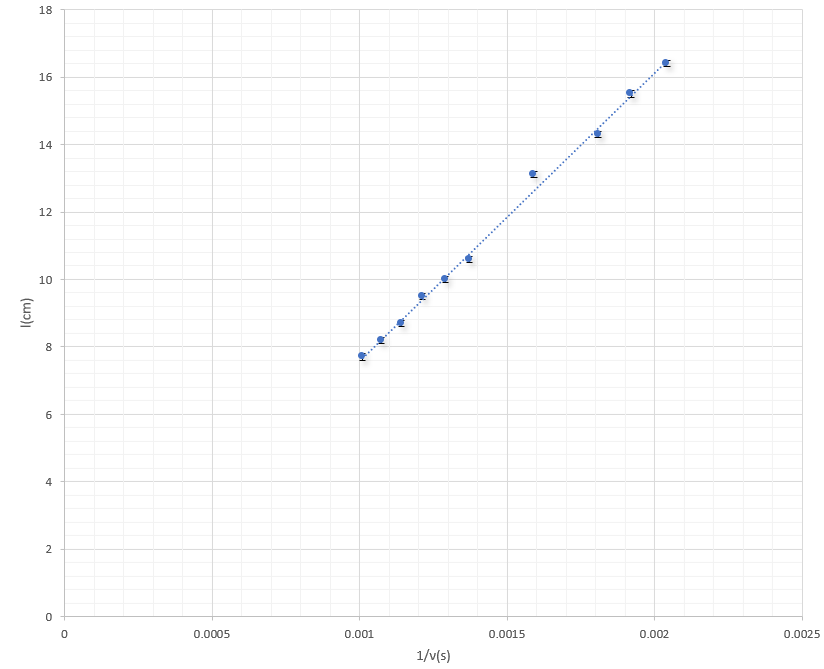
\includegraphics{1.PNG}
\caption{The speed of sound measurements fitted to an equation of y=mx+c where $m = 8548.4 cm s^{-1}, c=-0.96075 cm$}\label{1png}
\end{figure}

\subsection{Assume k is precisely known (columns M,N)}
However, if the value of d is very well measured and has negligible error associated with it, then $c$ will need to be fixed at the exact value of $c=-0.3d=-0.855$cm, so that there will only be 1 degree of freedom to consider ($\frac{\partial \chi^2}{\partial m} = 0$ only), massively simplifying the problem which becomes trivial to calculate.

Alternatively, one can use the covariance values obtained to calculate the new m expected to be obtained:

Forcing $c$ to equal $0.3 \times 2.85$ cm gives 
\begin{align}
	\Delta & m = m_{new} + m_{opt}\\
	\Delta & c = c_{new} + c_{opt}
\end{align}
where $c_{new}= 0.3 \times 2.85$, $m_{opt}, c_{opt}$ are the optimal values of c previously calculated by the method above without applying any constraints.

\begin{align}
	slope \: of \: regression = \bigg( \frac{cov(m,c)}{\sigma_c^2} \bigg)
\end{align}

By shifting c to the right (or in this case where $\Delta c$ is negative, left) by $\Delta c$, the corresponding value of m will go up changed by the following equation:

\begin{align}
	\Delta m = \bigg( \frac{cov(m,c)}{\sigma_c^2} \bigg) \Delta c
\end{align}

This displaces the coordinates of the fitting parameters $(m,c)$ from their optimal coordinates $(m_{opt},c_{opt})$ where the global minimum of $\chi^2$ exist; instead arrives at the point $m_{new},c_{new}$ which has a slightly higher $\chi^2$. The resulting errors on $m,c$ ($\sigma_m, \sigma_c$) should deviate from the original values $\sigma_{m_{opt}}, \sigma_{c_{opt}}$ found at the global minimum $(m_{opt},c_{opt})$; but can be approximated (to the $1^{st}$ order) as the original errors ($\sigma_{m_{new}}=\sigma_{m_{opt}}, \sigma_{c_{new}}=\sigma_{c_{opt}}$) (see N19 and N20).

The spreadsheet has been laid out in such a way that entire rows of data can be deleted to remove data points which appears to be outliers (while still accounting for a correct number of degree of freedom).

For example, row 6 containing the data point which is 27.3 standard deviations away from the expected value ($\chi^2$ contribution $= 27.3$) can be deleted, reducing the $\frac{\chi^2}{DoF}$ value from 4.95 to 1.24

\section{F.1: arcsin differentiation}
\begin{align}
  D &= \frac{ln(1+\Delta)}{h}  							\\
  D_{1^{st}order}  &= \frac{1}{h} (\Delta)                      \label{1storder} \\
  D_{2^{nd}order}  &= \frac{1}{h} [\Delta-\frac{\Delta^2}{2}]   \label{2ndorder}
\end{align}
where

$D$ = Differential operator = $\frac{d}{dx}$

$\Delta$ = Forward difference operator, the result of application of which is shown in column C;

$h$ = mesh-spacing = $0.01$

Equation \ref{1storder} and \ref{2ndorder} are truncated to $1^{st}$ and $2^{nd}$ order respectively in column E and F.

\subsection{fractional error}
If the analytical solution to the differential equation is known, then the fractional error of the numerical answers obtained by the $1^{st}$ and $2^{nd}$ order expansion are respectively calculated by equation \ref{err1} and \ref{err2} below:
\begin{align}
\Delta D_1 &= \frac{D_{1^{st}order}f-f'(x)}{f'(x)} \label{err1}\\
\Delta D_2 &= \frac{D_{2^{nd}order}f-f'(x)}{f'(x)} \label{err2}
\end{align}
The result of evaluating expression \ref{err1} and \ref{err2} are shown in column H and I respectively.

\begin{figure}[!h]
\centering
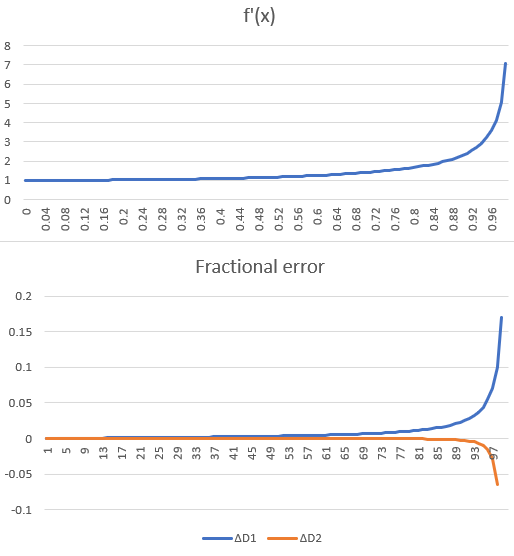
\includegraphics{2.PNG}
\caption{The fractional error when differentiating arcsine using the forward operator, without(blue) and with(orange) 2nd order corrections applied. The analytical solution for f'(x) is plotted directly above for reference.}\label{2png}
\end{figure}

\subsection{arcsin}

For the specific case in question

\begin{align}
f'(x)=\frac{d}{dx}sin^{-1}(x)=\frac{1}{\sqrt{1-x^2}}
\end{align}
This analytical result is shown in column G

\section{G.2: Breit-Wigner integration}

\subsection{Simpson's Rule}
\begin{align}
I=\frac{h}{3}[f_0+\sum\limits_{i=1}^{N-1}(4f_{2i-1}+2f_{2i}) + 4f_{2N-1}+f_{2N}]
\end{align}
where the 4/2 in front of the odd/even terms are declared in the "multiplication factor" column (D), so that they can be multiplied together in the "sum" column (E) and then summed at the bottom of it (cell E24).
\subsection{Gaussian Quadrature}

\begin{figure}[!h]
\centering
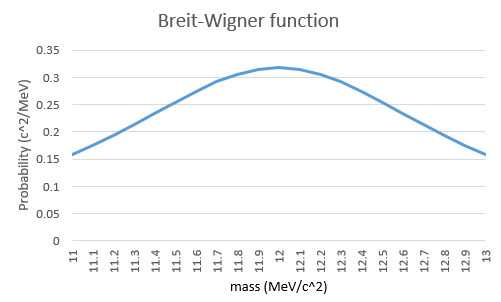
\includegraphics{3.PNG}
\caption{Breit-Wigner function in the region of interest}\label{3png}
\end{figure}

\begin{align}
  I&= \int\limits_{-1}^{1} g(\theta) d\theta  = \int\limits_{a}^{b} f(x) dx \\
   &\approx \sum \limits_{i=1}^{2} [g(\theta_1)-g(-\theta_1)] w_i \label{GaussSummation}
\end{align}
Note the symmetricality of the distribution in Figure \ref{3png}. In fact it is an even function about $x=12$, which allows the integration limits to be changed to $a=12,b=13$ instead.

In equation \ref{GaussSummation} the value of $\theta$, as provided by the assignment pdf, are listed in column G. The weight factor $\omega$ are listed in column H.
The range to be integrated (in $f(x) space$) is then mapped onto the range between $-1$ and $1$ (in $g(\theta)$ space)
\begin{align}
  x \in [a=12,b=13] \mapsto \theta \in [-1,1] \label{mapsto}
\end{align}
and then integrated over -1 to 1 via the equation \ref{GaussSummation}, requiring a scale factor of $\frac{\Delta x}{1-(-1)} = \frac{\Delta x}{2}$ to be multiplied when carrying out the summation in equation \ref{GaussSummation} (see column I).

The inverse of the transformation in equation \ref{mapsto} from $\theta$ space into $x$ space is shown in column K, allowing the value of $f(x)$ to be computed; and then it is transformed back into $g(\theta)$ space in column I. It is weighted and summed as stated in equation \ref{GaussSummation} in column J.

\section{J.4: Curve of Persuit}
\subsection{Analytical solution of the trajectory}
Using the shorthand of $\beta=\frac{v_b}{v_a}$, the analytical solution of y is evaulated as follows:
\begin{align}
	y= \int q dx &=\int \limits_0^x \frac{1}{2} [(1-\frac{x'}{d})^{-\beta} - (1-\frac{x'}{d})^\beta]  dx' \\
	&=\frac{d}{2} \int\limits_0^x [(1-\frac{x'}{d})^{-\beta} - (1-\frac{x'}{d})^\beta] d(1-\frac{x'}{d})
\end{align}
Using the shorthand of $\mu=(1-\frac{x'}{d})$:
\begin{align}
	y&= -\frac{d}{2} \int\limits_0^x (\mu^{-\beta} - \mu^\beta) d\mu \\
	&= -\frac{d}{2}  \big[ \frac{\mu}{1-\beta} \mu^{-\beta} - \frac{\mu}{\beta+1} \mu^\beta \big]_0^x \\
	&= \frac{d}{2} \big[ \mu \frac{(\beta+1)\mu^{-\beta}+(\beta-1)\mu^\beta}{(\beta^2 -1)} \big]_0^x
\end{align}
where for $x'=0, \mu=1$ as long as $d\neq 0$, so the integral's lower limit evaluates to 
	
\begin{align}
lower\: limit=\frac{d}{2} \frac{2\beta}{\beta^2 -1} = \frac{d\beta}{\beta^2 -1} \label{GeneralLowerLimit}
\end{align}
for $\beta=\frac{1}{3} , d=50$ this evaluates to 
\begin{align}
lower\: limit = -\frac{9(50)\frac{1}{3}}{8} = -\frac{150}{8}
\end{align}
This gives the result
\begin{align}
	y&=\frac{d}{2} \bigg[ \frac{\mu^{1-\beta}} {\beta -1} + \frac{\mu^{1+\beta}} {\beta +1} \bigg] - lower\: limit  \label{GeneralAnalytic}\\
	&= \frac{50}{2} \bigg[ \frac{\mu^{\frac{2}{3}}} {-\frac{2}{3}} + \frac{\mu^{\frac{4}{3}}} {\frac{4}{3}} \bigg] + \frac{150}{8}\\
	&= \frac{150}{8} \bigg( -2\mu^{\frac{2}{3}} + \mu^{\frac{4}{3}} + 1 \bigg)
\end{align}
where
\begin{align}
	\mu=(1-\frac{x}{d})=(1-\frac{x}{50})
\end{align}
Equation \ref{GeneralAnalytic} is used in conjunction with \ref{GeneralLowerLimit} in column AF to give the analytical solution.

\subsection{Runge-Kutta method}
By applying the $4^{th}$ order Runge-Kutta method, using the following set of equations
\begin{align}
	\begin{cases}
		y'(x)= f(x,y,q)\\
		q'(x)= u(x,y,q)
	\end{cases}
\end{align}
	where, using the same notations as above ($\mu =(1-\frac{x}{d})$ and $\beta = \frac{v_b}{v_a}$),
\begin{align}
	\begin{cases}
		f(x,y,q) = f(x) = q(x) = \frac{1}{2} [ \mu^{-\beta} - \mu^{\beta}] \\
		u(x,y,q) = u(x,q) = -\beta \frac{\sqrt{1+q^2}}{(x-d)}
	\end{cases} \label{qEquation}
\end{align}
at each meshpoint, $y_i' = y'(x_i), q_i' = q'(x_i)$
\begin{align}
	\begin{cases}
		y_{i+1} - y{i} = y(x_i+h) - y(x_i) = \frac{1}{6} (k_0 +2k_1 + 2k_2+k_3) \\
		q_{i+1} - q{i} = q(x_i+h) - q(x_i) = \frac{1}{6} (g_0 +2g_1 + 2g_2+g_3)
	\end{cases} \label{IncrementEquation}
\end{align}
\begin{align}
	\begin{cases}
		k_0= hf(\vec{r}_0), g_0 = hu(\vec{r}_0)\\
		k_1= hf(\vec{r}_1), g_1 = hu(\vec{r}_1)\\
		k_2= hf(\vec{r}_2), g_2 = hu(\vec{r}_2)\\
		k_3= hf(\vec{r}_3), g_3 = hu(\vec{r}_3)\\
	\end{cases}
\end{align}
\begin{align}
	\begin{cases}
		\vec{r}_0^T = (x_i, y_i, q_i) \\
		\vec{r}_1^T = (x_i+\frac{h}{2}, y_i+\frac{k_0}{2}, q_i+\frac{g_0}{2}) \\
		\vec{r}_2^T = (x_i+\frac{h}{2}, y_i+\frac{k_1}{2}, q_i+\frac{g_1}{2}) \\
		\vec{r}_3^T = (x_i+h, y_i+k_2, q_i+g_2)
	\end{cases}
	\label{MeshpointCoordinates}
\end{align}
\begin{itemize}
	\item For each mesh point;
	\begin{itemize}
		\item The coordinates $\vec{r_i}$ is evaluated, ($\vec{r}^T = (x,y,q)$ as stated in equation \ref{MeshpointCoordinates}; but $y$ does not need to be explicitly evaluated because there is no y-dependence in any of the equations). \\
		These coordinates ($x_i,q_i$) are stored on the \underline{\textbf{rightmost}} two columns of each coloured text box. (columns G, H, M, N, S, T, Y, Z)
		\item The functions $f(\vec{r_i}) = q(x_i)$ and $u(\bar{r_i}) = \frac{dq}{dx} (x_i,q_i) $ are evaluated at these coordinates, and their values are stored in the \underline{\textbf{central}} two columns of each coloured text box. (columns E, F, K, L, Q, R, W, X)
		\item The incremental values $k_i = hf(\vec{r_i}) $ and $g_i = hu(\bar{r_i})$ are evaluated and stored on the \underline{\textbf{leftmost}} two columns of each coloured text box. (columns C, D, I, J, O, P, U, V)
	\end{itemize}
	\item The resulting incremental values $g_j$ and $k_j$ for $j=\{ 0,1,2,3 \}$ are added together in their respective weighted sums AA and AD respectively. They are then added onto the existing value \underline{\textbf{in the next row}} in column AB and column AE.
	\item The deviation of the computed value of y from its analytical solution increases monotonically, accelerating as the value of y increases more and more quickly towards the point of convergence. \\
	However, this trend is temporarily arrested by the decrease in step size (h), thus showing that smaller step size improves precision. \\
	The same trend as described above applies for the deviation of q from its analytical value.
	\item At the point of contact, $y(x=d=50)$, q approaches infinity as $ (1-\frac{x}{d}) =\mu \to 0$, so $\mu^{-\beta} \to \infty$, so when finding the increment that leads up to x=50 (equation \ref{IncrementEquation}) , the value of $k_3$ approaches infinity due to $\mu$ approaching 0 in equation \ref{qEquation}
\end{itemize}

\end{document}